\section{MLPs training}\label{sec:mlptraining}

Script \texttt{mlptrain.m} performs the training of both networks using the
architectures selected in \secref{subsec:mlpbayesopt} and the training
algorithms and feature extraction methods selected in
\secref{subsec:mlphyperopt}.

\vfigref{fig:mlptrainperformance} shows the training performance plots for both
networks. 

\begin{figure}[htbp]
	\centering
	\begin{subfigure}{\textwidth}
		\centering
		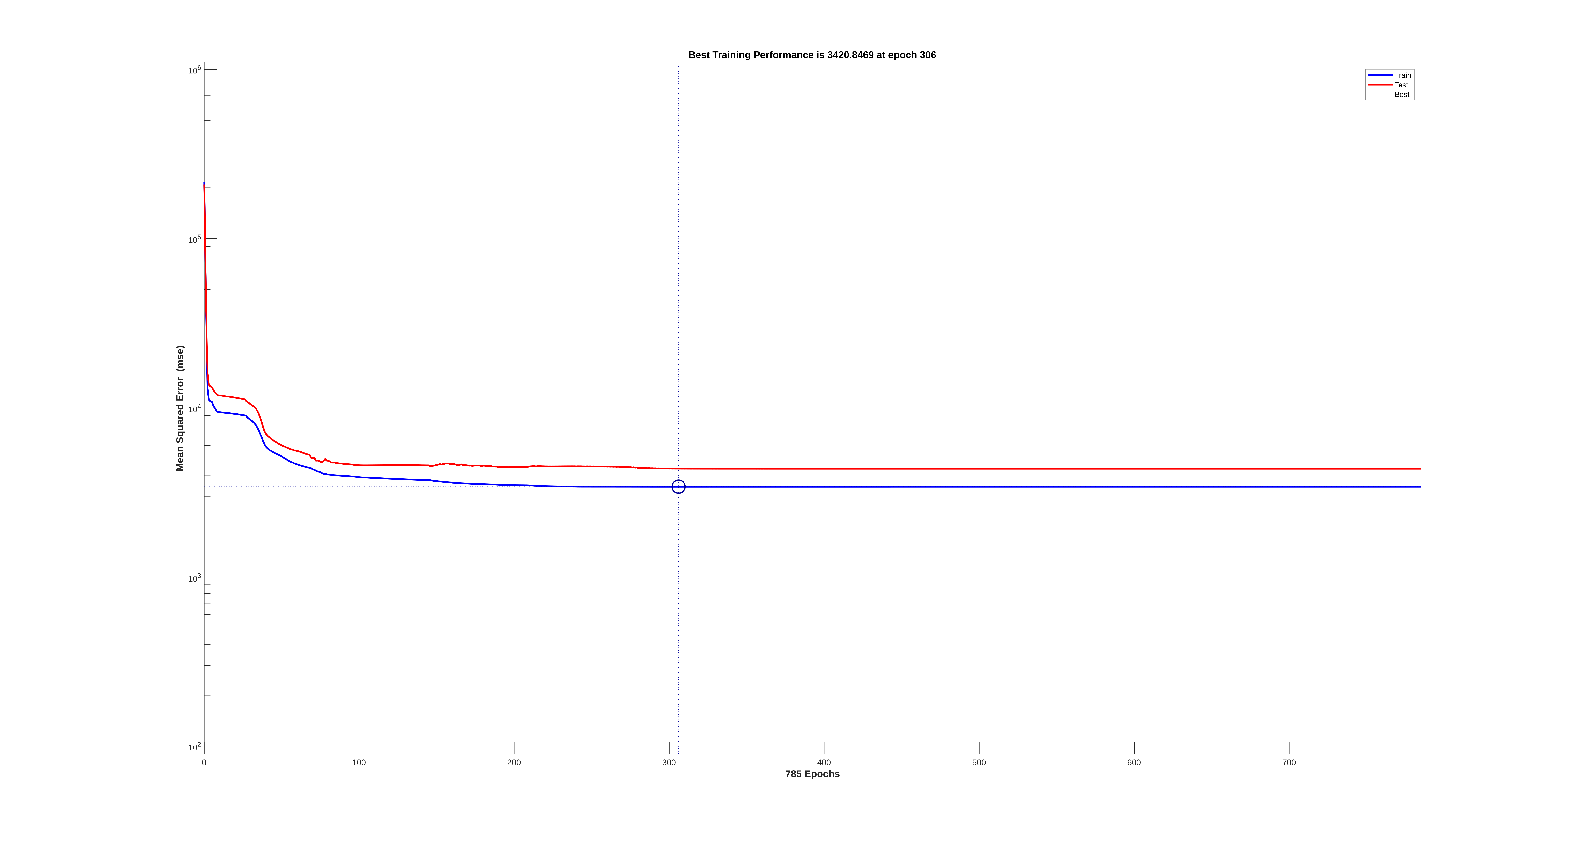
\includegraphics[width=\textwidth, trim=2.95cm 1.1cm 2cm 0.8cm,
		clip]{mlpmeantrainperformance}
		\caption{Training performance plot for the ECG's mean
		estimation network.}\label{fig:mlpmeantrainperformance}
	\end{subfigure}
	\begin{subfigure}{\textwidth}
		\centering
		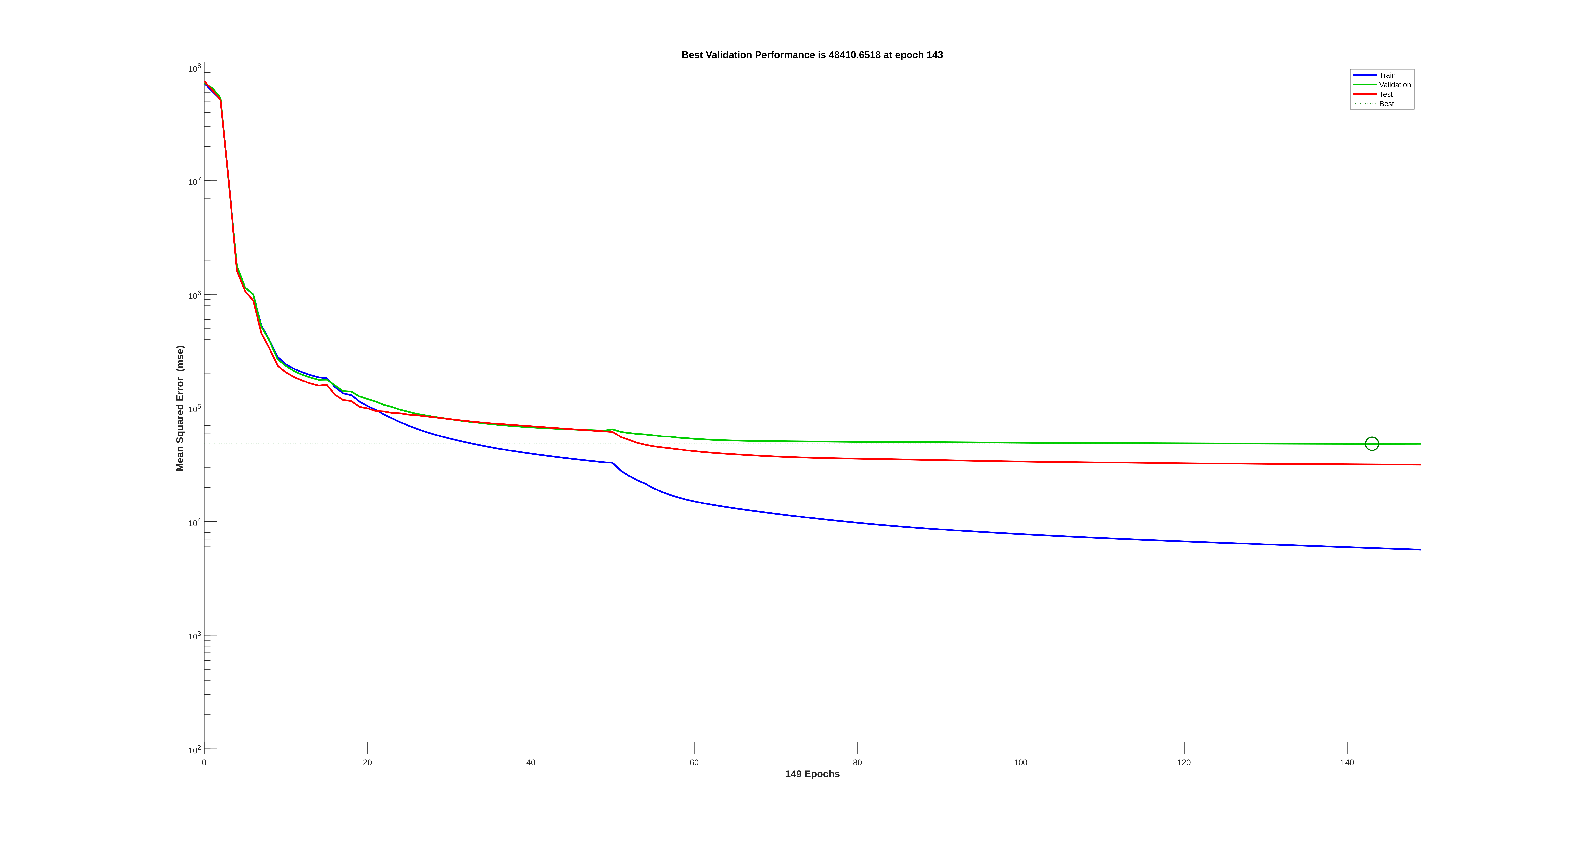
\includegraphics[width=\textwidth, trim=2.95cm 1.1cm 2cm 0.8cm,
		clip]{mlpstdtrainperformance}
		\caption{Training performance plot for the ECG's standard
		deviation estimation network.}\label{fig:mlpstdtrainperformance}
	\end{subfigure}
	\caption{Training performance plots for the two
	networks.}\label{fig:mlptrainperformance}
\end{figure}

\vfigref{fig:mlpstdregression} shows the regression plot for the ECG's standard
deviation estimation network. The network performs very well, with a
coefficient \(R = 0.99184\) for the test set and \(R = 0.99616\) for the entire
dataset.

\begin{figure}[htbp]
	\centering
	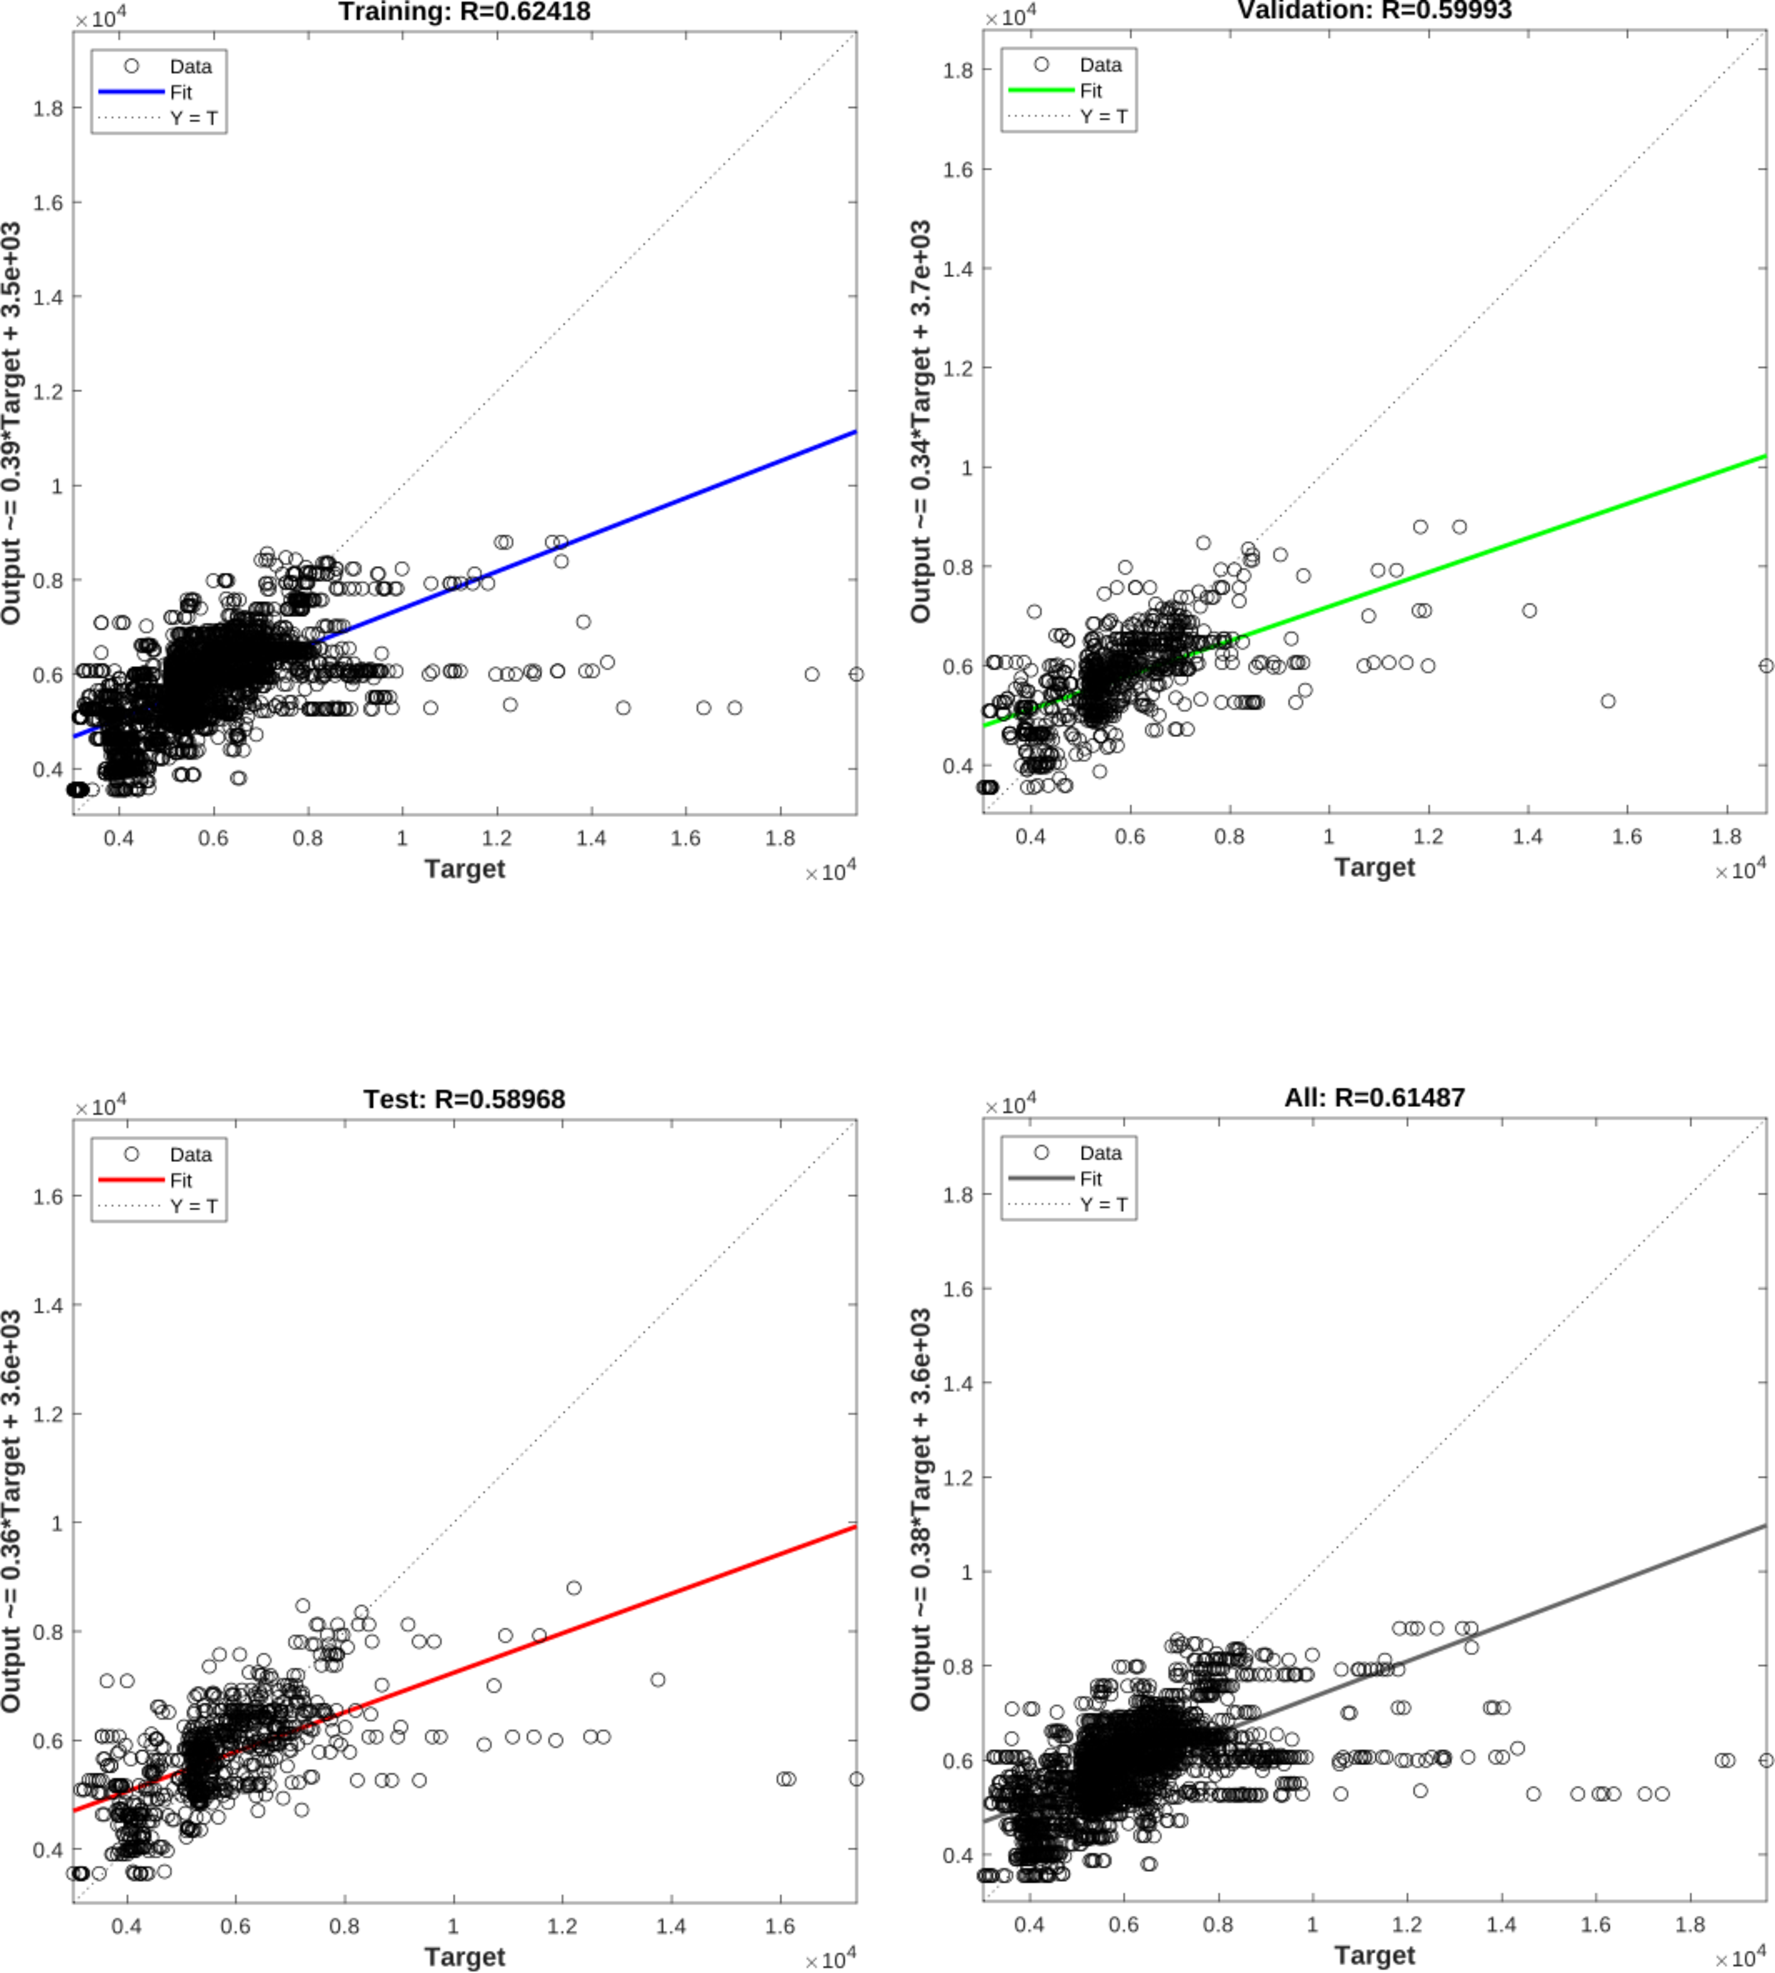
\includegraphics[width=\textwidth]{mlpstdregression}
	\caption{The regression plot for the ECG's standard deviation
	estimation network shows excellent
	results.}\label{fig:mlpstdregression}
\end{figure}

The ECG's mean estimation network performances are not so good (but still
valuable), as shown in \vfigref{fig:mlpmeanregression}: we have \(R = 0.85045\)
for the test set and \(R = 0.85761\) for the entire dataset. This latter
network will be the subject of \chref{ch:cnn}.

\begin{figure}[htbp]
	\centering
	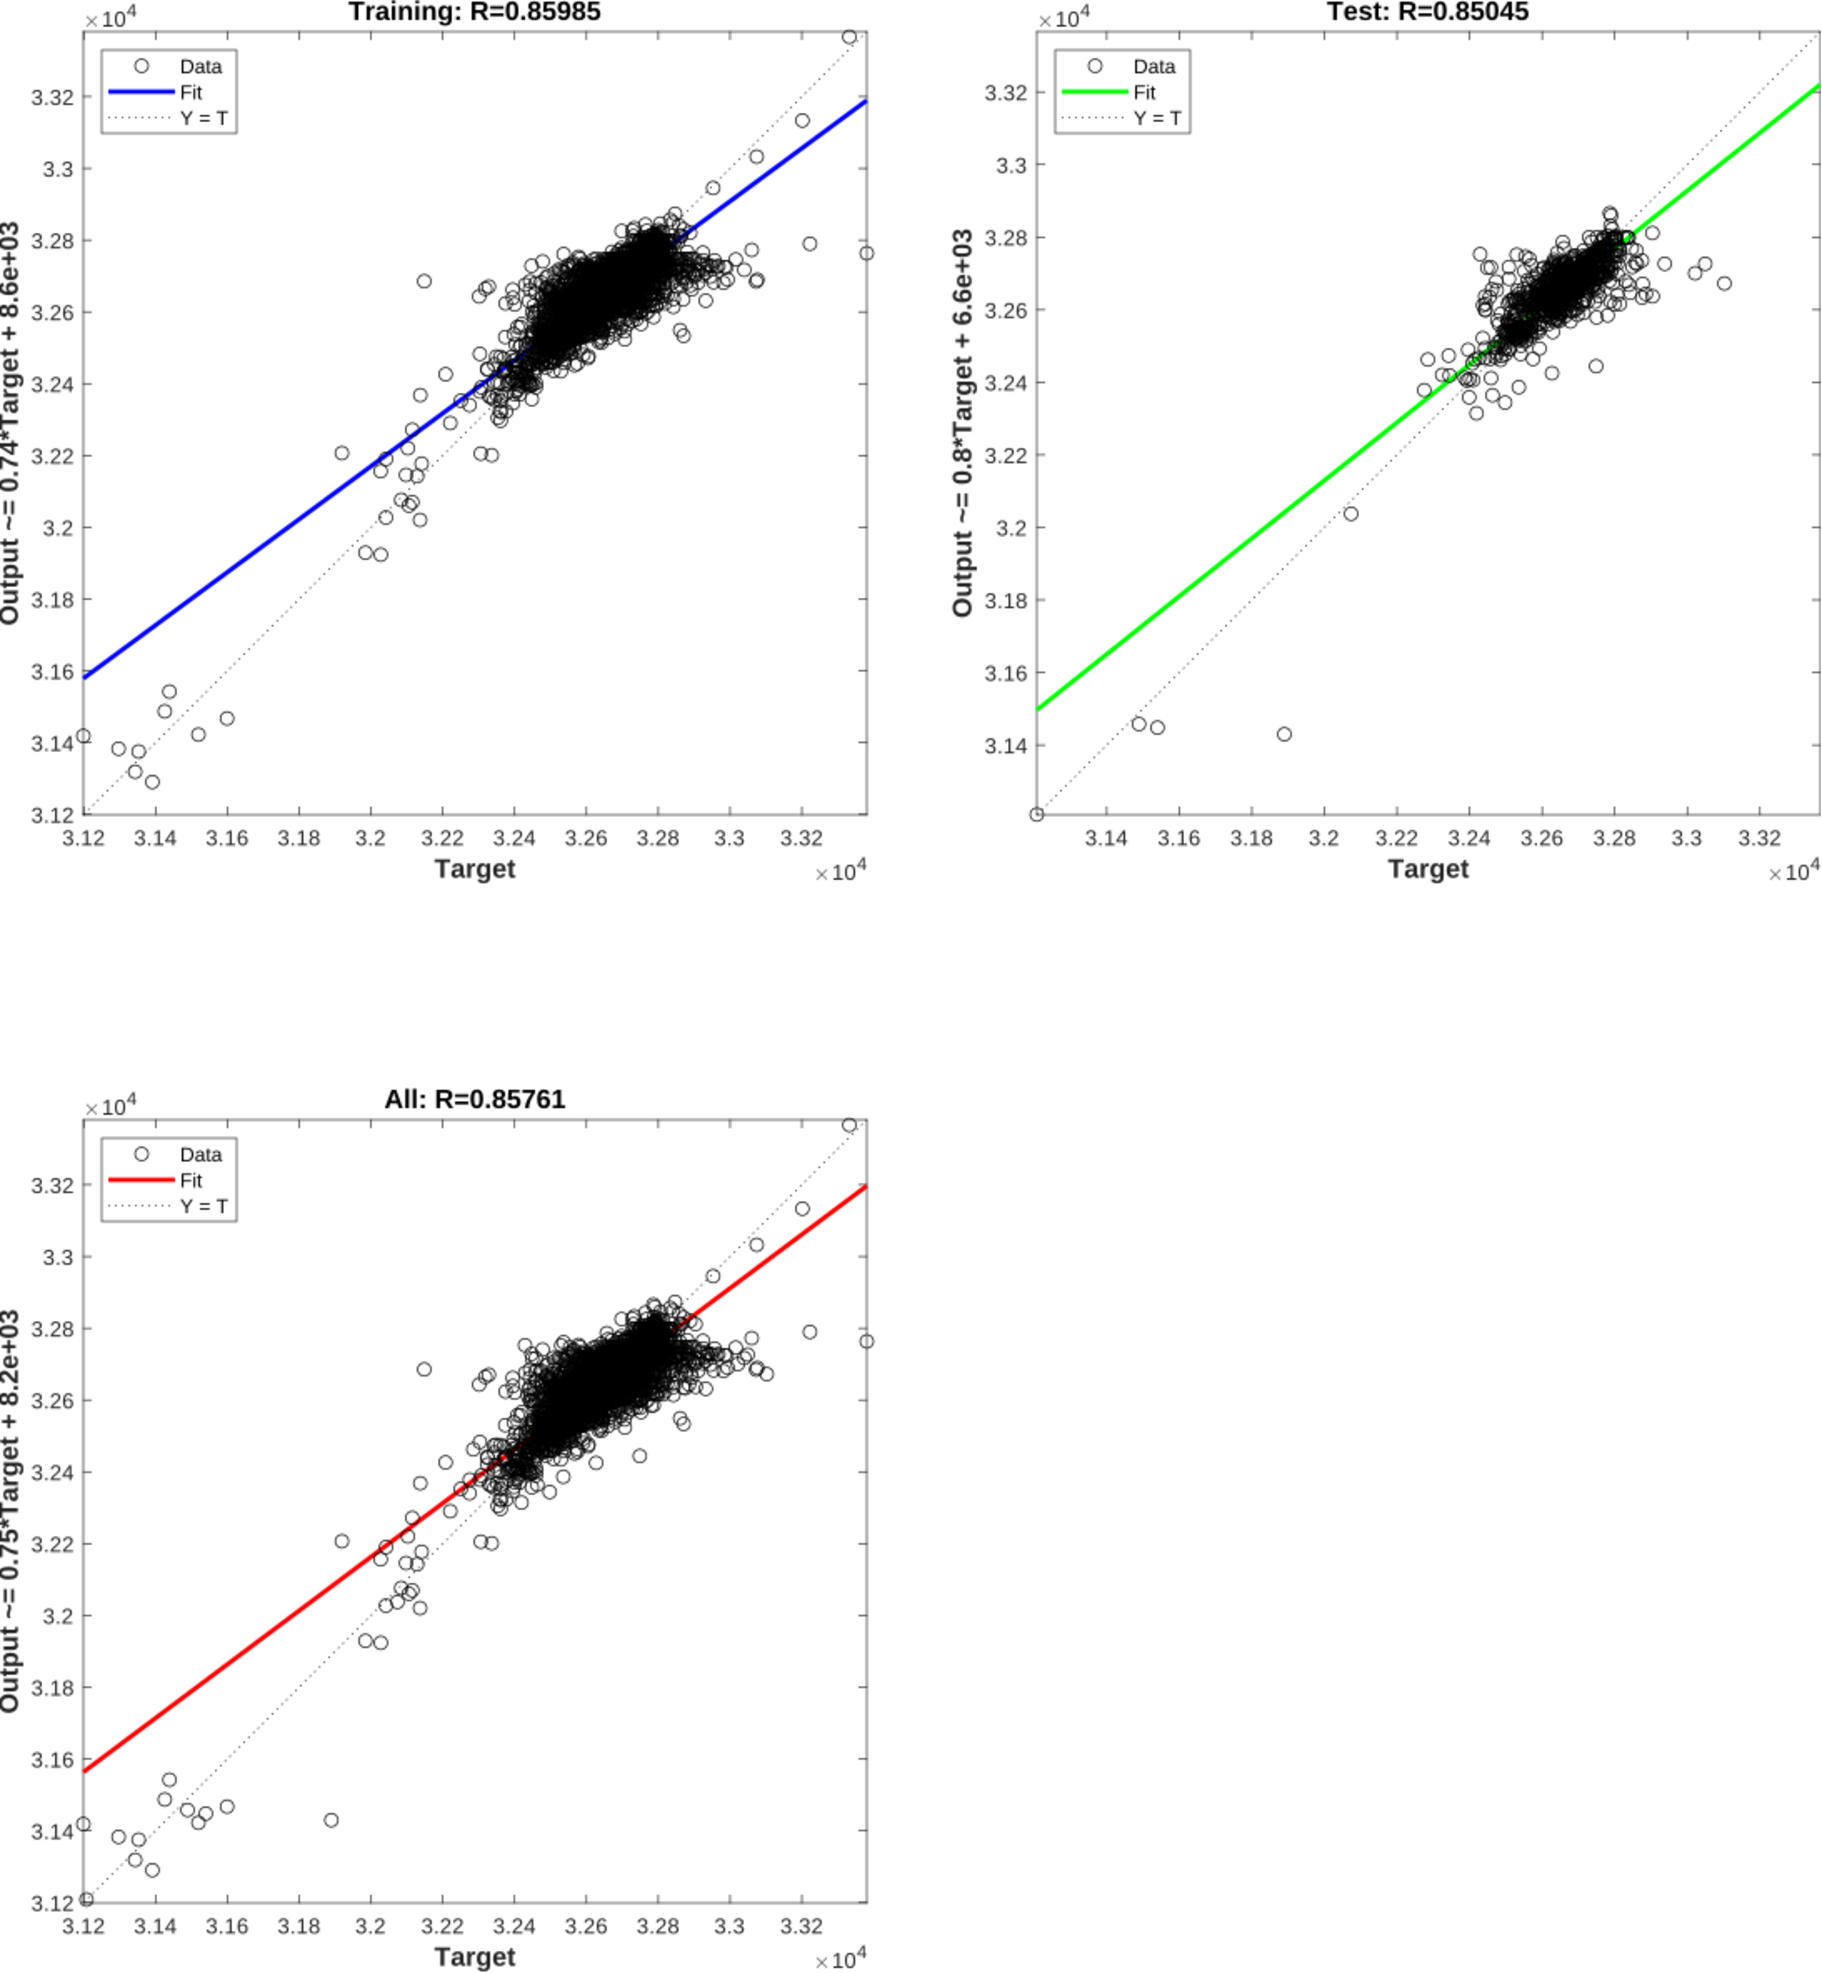
\includegraphics[width=\textwidth]{mlpmeanregression}
	\caption{The regression plot for the ECG's mean estimation network
	shows good, but not excellent, results.}\label{fig:mlpmeanregression}
\end{figure}

\vfigref{fig:mlperrorhists} shows the error histograms for both networks.

\begin{figure}[htbp]
	\centering
	\begin{subfigure}{\textwidth}
		\centering
		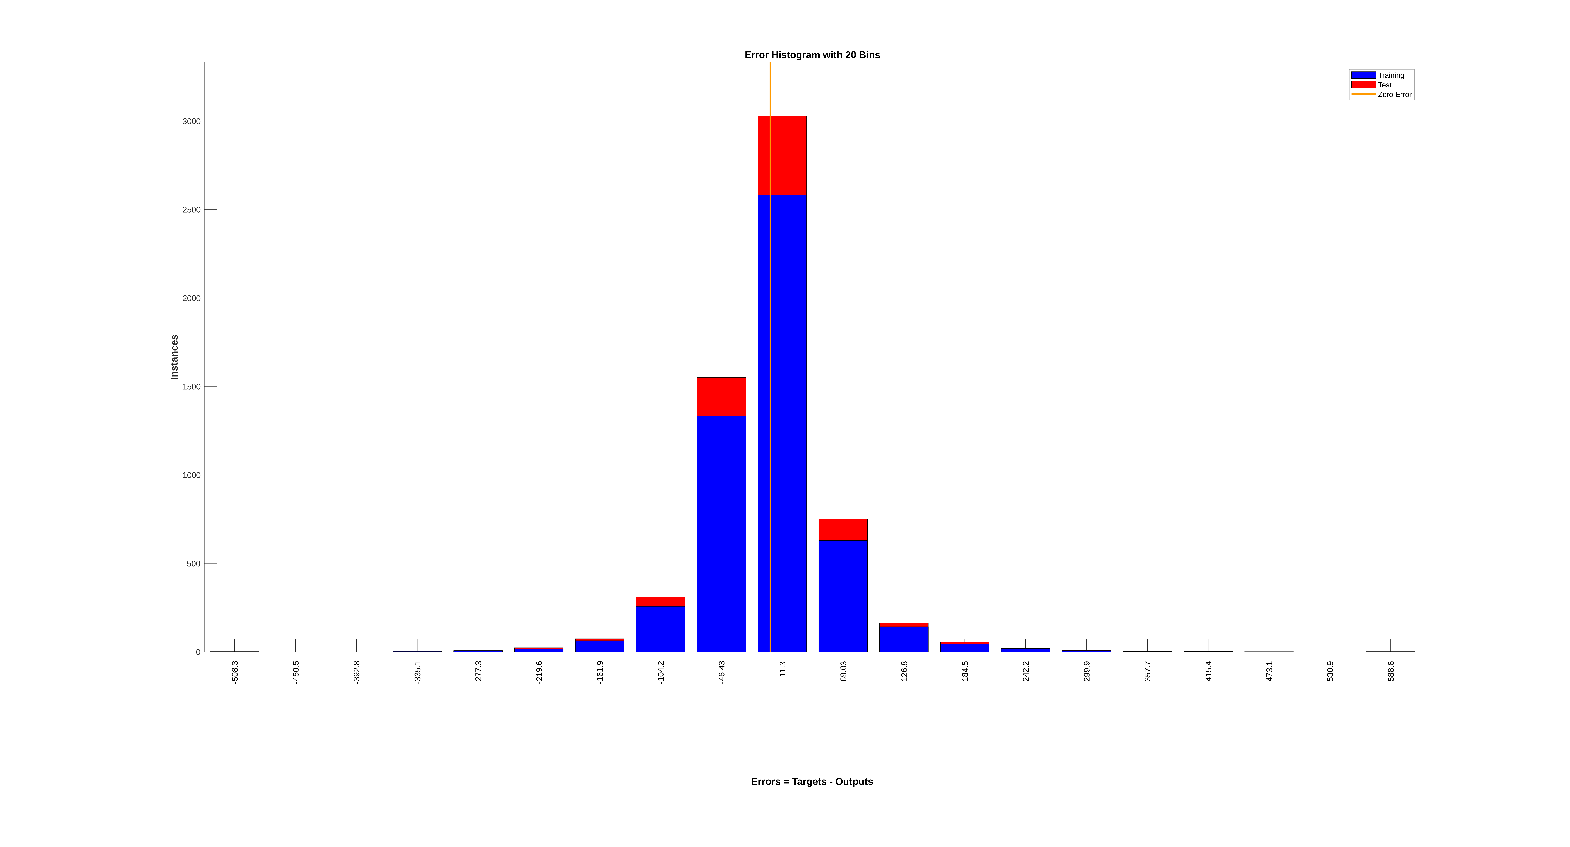
\includegraphics[width=\textwidth, trim=2.9cm 1cm 2cm 0.8cm,
		clip]{mlpmeanerrorhist}
		\caption{Error histogram for the ECG's mean estimation
		network.}\label{fig:mlpmeanerrorhist}
	\end{subfigure}
	\begin{subfigure}{\textwidth}
		\centering
		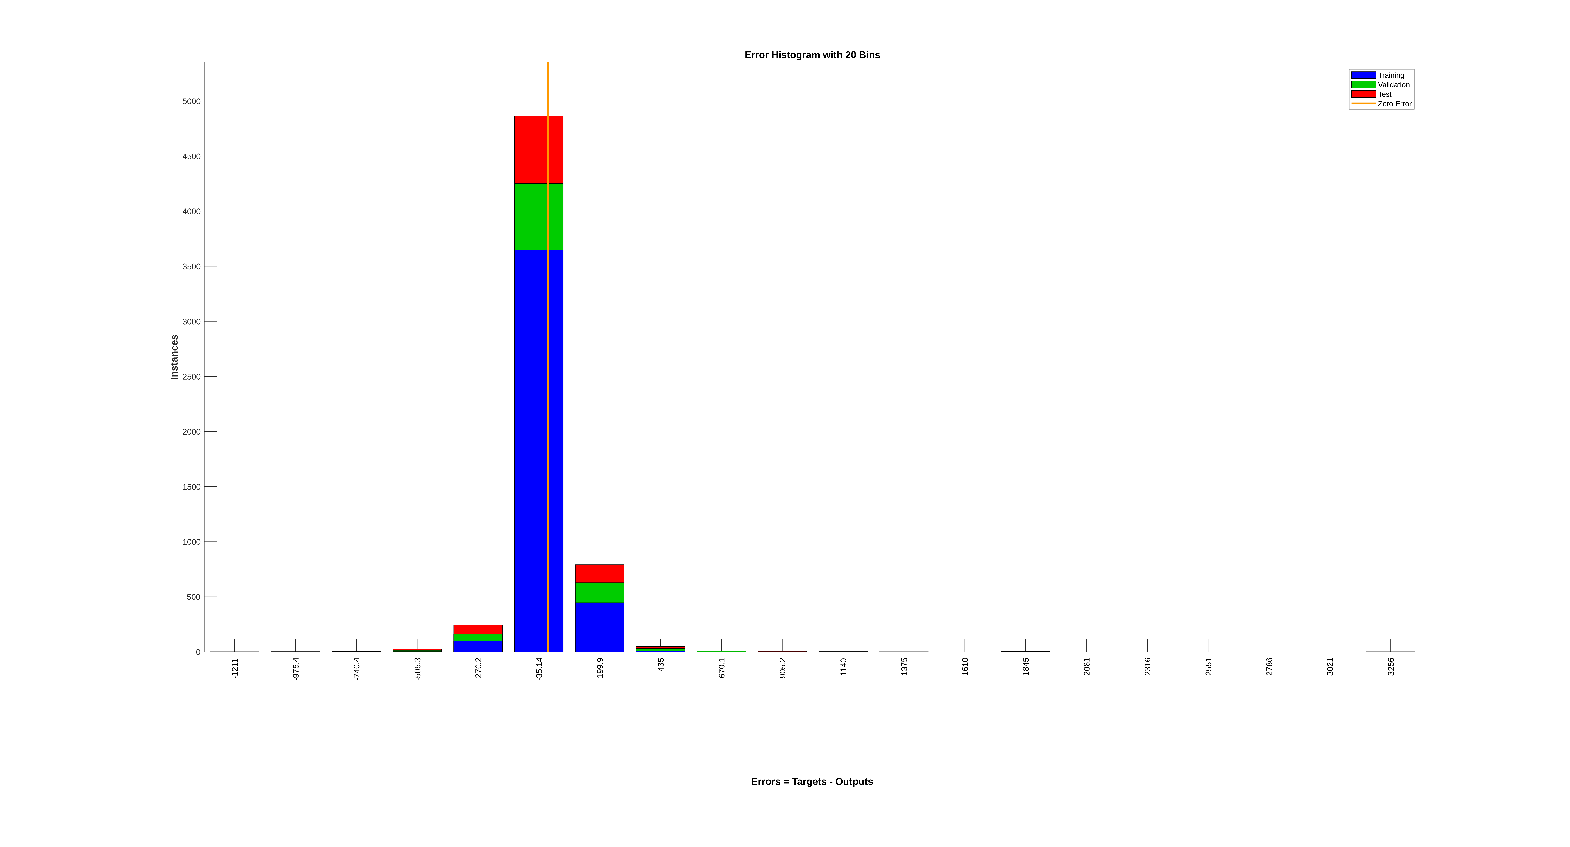
\includegraphics[width=\textwidth, trim=2.9cm 1cm 2cm 0.8cm,
		clip]{mlpstderrorhist}
		\caption{Error histogram for the ECG's standard deviation
		estimation network.}\label{fig:mlpstderrorhist}
	\end{subfigure}
	\caption{Error histograms for the two
	networks.}\label{fig:mlperrorhists}
\end{figure}
